\documentclass[12pt,a4paper]{article}

% PAPER TITLE
\newcommand{\asgtitleshort}{Graph ECS}
\newcommand{\asgtitlelong}{A Graph Based Approach To Concurrent ECS Design}

% NAME
\newcommand{\nameshort}{Emil}
\newcommand{\namelong}{E.D Choparinov}

\usepackage[T1]{fontenc}
\usepackage{fontspec}
\defaultfontfeatures{Ligatures=TeX}

\usepackage{biblatex}
\bibliography{paper/refs.bib}

\usepackage{amsthm}
\usepackage{thmtools}
\usepackage{amsmath}
\usepackage{amsfonts}
\usepackage{amssymb}
\usepackage{textcomp,gensymb}
\usepackage{tikz}
\usetikzlibrary{arrows,automata}

\usepackage{algorithm}
\usepackage{algpseudocode}
\usepackage{minted}
\usepackage{xcolor}
\usepackage{csquotes}

\usemintedstyle{perldoc}

\usepackage{graphicx}
\usepackage{wrapfig}
\usepackage{caption}
\usepackage{subcaption}

\usepackage{hyperref}

\setlength{\textwidth}{16cm}
\setlength{\textheight}{22.5cm}
\setlength{\topmargin}{-2cm}
\setlength{\oddsidemargin}{0cm}
\setlength{\evensidemargin}{0cm}
\setlength{\parindent}{5mm}

\usepackage{color}
\definecolor{darkred}{rgb}{0.6,0.0,0.0}
\definecolor{darkgreen}{rgb}{0,0.50,0}
\definecolor{lightblue}{rgb}{0.0,0.42,0.91}
\definecolor{orange}{rgb}{0.99,0.48,0.13}
\definecolor{grass}{rgb}{0.18,0.80,0.18}
\definecolor{pink}{rgb}{0.97,0.15,0.45}

% listings
\usepackage{listings}

% Code definition
\lstset{
  aboveskip=1em,
  breaklines=true,
  abovecaptionskip=-6pt,
  captionpos=b,
  frame=single,
  numbers=left,
  numbersep=15pt,
  numberstyle=\small,
  showstringspaces=false
}


% Code color theme definition
\lstdefinestyle{colored}{ %
  basicstyle=\ttfamily,
  backgroundcolor=\color{white},
  commentstyle=\color{darkgreen},
  keywordstyle=\color{blue}\bfseries\itshape,
  stringstyle=\color{red},
  morekeywords={A,B,C}
}

% Theorem Defintions
\colorlet{shadecolor}{white}
\newtheorem{thm}{Theorem}

\newtheoremstyle{definitionsty}{15pt}{15pt}{\slshape}{}{\bfseries}{.}{.5em}{}
\theoremstyle{definitionsty}
\newtheorem{tdefn}{Definition}
\newenvironment{defn}
  {\begin{shaded}\begin{tdefn}}
  {\end{tdefn}\end{shaded}}

\usepackage{blindtext}

\usepackage{fancyhdr}
\pagestyle{fancy}
\fancyhf{}
\usepackage{lastpage}

\setlength{\headheight}{65pt}
\rhead{\large \asgtitlelong}
\lhead{\large \namelong}
\rfoot{Page \thepage /\pageref{LastPage}}

\newcommand{\ZZ}{\mathbb{Z}}
\newcommand{\RR}{\mathbb{R}}

\author{\namelong}
\title{\asgtitlelong}
\date{\today}

\begin{document}

\maketitle

\thispagestyle{fancy}
\begin{abstract}
  The Entity Component System, also known widely as ECS, is the most important architectural design pattern for realtime simulations. By decoupling data from logic, ECS architectures uniquely excel at faciliting compositions of dynamic objects. The objective of this thesis is split into four parts. 

  The study begines with an introduction and literature review of the ECS pattern, highlighting its strengths and weaknesses, and includes the motivation as to why to use an ECS over Object-Oriented Programming in realtime simulation contexts. The paper will then move on to a review of the implementation styles noticed while researching various real-world ECS implementations. Chapter \ref{chap:1} concludes with touching broadly on the concurrency styles those real-world ECS's used in their implementations.
  
  Chapter \ref{chap:2} is dedicated to the concurrency techniques used in the GECS library, the ECS implemented for this paper. The introduction begins by discussing the topic of vectorization and rethinking about components as types and archetypes. It then explores using archetypes to construct a runtime entity finite-state-machine (FSM) to aid in scheduling the ECS in concurrent contexts. Before wrapping up the chapter, it touches on how to retain validity of the entity FSM over runtime.
  
  Chapter \ref{chap:3} finally introduces the GECS library implemented for this paper. This chapter covers all topics related to implementation details to data layout and the structures used. Preserving the vectorizability of archetypes and the concurrency implementation are explained in greatest detail. The remainder of this paper is benchmarking and discussions of the results following from implementing GECS. 

  GECS aims to optimize for execution in general purpose scripting contexts from performing physics calculations to facilitating user interactions. It's important to note before reading futher on that due to the nature of this subject, scientific journals regarding this topic is limited. However, articles about designing ECS architectures and presentations are widely availabile online from reputable organizations.

  Experimental results are **TDB**
\end{abstract}

\newpage

\newpage
\tableofcontents
\newpage

\section{ECS Literature Review}
\label{chap:1}

Historically, realtime interactive systems like simulations and game development have relied on object-oriented design techniques which introduced massive class hiearchies, deep inheritance paths, and highly specialized code to projects. The aim of an ECS is to allievate, or downright remove, many of the negatives that come with classical object-oriented design. ECS architectures follow the composition over inheritance principle, which aims to manage entities in large scale real-time applications efficiently. \cite{Haerkoenen2019} 

\subsection{Entity Component System Foundations}
These are the foundational definitions used in this paper.

\subsubsection{Entity}
    An entity is a unique identifier used to represent a "thing" in the simulation. This unique identifier is used in some manner by the ECS to collect a set of components. Some ECS's try to make the identifier intelligent to optimize component selection by using the bytes in an integer to store more location information. This will be discussed in the existing ECS implementions.

\subsubsection{Component}
    Generally speaking, a component is data. It can be defined as a struct, tuple, or class. For this thesis, we define a component to only be a segment of either complete or incomplete data.

\subsubsection{Tag}
    A tag is a component such that it contains 0 information other than its existence.

\subsubsection{System}
    A system has two parts. First the query and second the execution. A system queries for a collection of components and then executes a function that can modifies, create, or destroy entities or components.

\subsubsection{Tick}
    A tick is defined to be a point during runtime in which all systems have been processed and the ECS is ready to process them all again. A tick is the serialization point of a concurrent ECS architecture.

\noindent The paper will build upon these four concepts and introduce new definitions based on these.

\subsection{The Weaknessess Of Object Oriented Programming}

% TODO: Sources
It has been exhaustively shown that Object-Oriented Programming (OOP) increases the difficulty of achieving desired simulation goals and that there are plenty attractive alternatives. The two main weaknesses that an ECS intends to solve is: poor cache utilization and poor parallelization.

Large projects deep into using OOP principles learn how hard it is to keep cached what you need and keep junk out. OOP principles can make pointer abuse very easy and cause the cache to overwrite potentially useful data in the near future. ECS solves this by introducing components. Since components are detached from their entity, we as engine designers can put these components wherever we please. It's not an uncommon practice to see component data be stored in long homogenous vectors. Suppose you have to do a heavy operation across the set of entities that all contain component $Q$. An ECS in this situation will be extremely cache friendly, due to $Q$ being next to components that all contain the same component type.

In OOP, parallelism can be painful due to synchronization errors over memory that was not engineered to effectively be parallelized. ECS follows principles from another design pattern called Data-Oriented Design (DOD). DOD, as a design theory, generally produces code that is more easily parallelizable. The concept of storing components as homogenous vectors not only helps with caching but because all data pertaining to a component is already in a homogenous vector -- it's easy to process in parallel or in groups.

\subsection{An Entity-Component System Model}

% TODO: NOTE, each thread gets a copy of this vector and we merge them at the first linearization point (next frame)
ECS Architectures are built upon two core data structures: vectors and hashmaps. The following architecture given is my naive ECS version. This example will not be thread safe and is purely for getting a taste of how different pieces of an ECS fit together.

\begin{figure}[htbp]
    \centering
    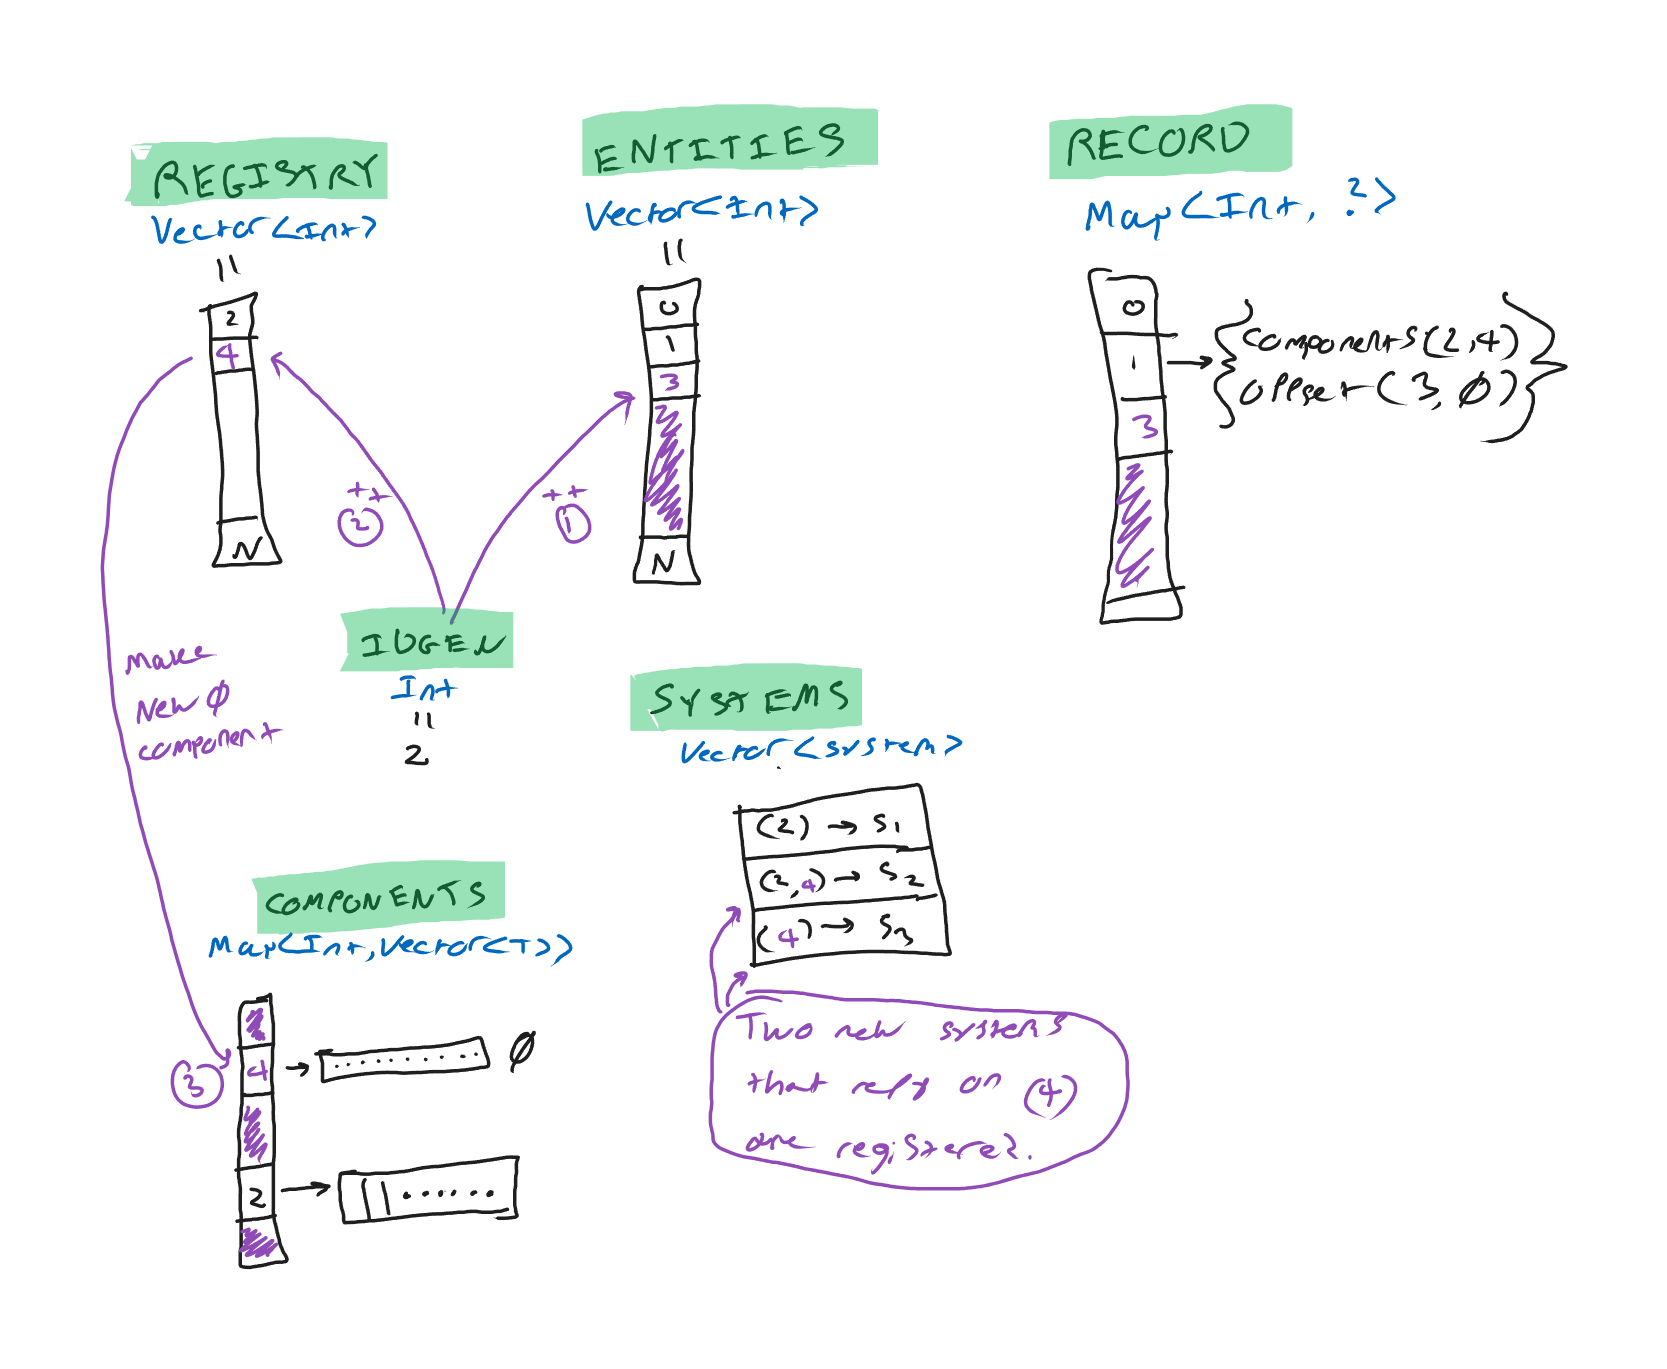
\includegraphics[width=0.5\linewidth]{resources/naive_ecs.png}
    \caption{Basic ECS Architecture Adding New Component}
    \label{fig:naive_ecs}
\end{figure}


There are a total of 6 major components to consider in this ECS model. 

\subsubsection{Entity}
The entity part is emulated via a variable IDGEN which is shared to generate unique identifiers for components and entities. This global variable is incremented each time an entity or component is generated. The list of active entities, stored in ENTITIES, is a list of uint64\_t values generated by IDGEN. 

\begin{figure}[H]
    \centering
    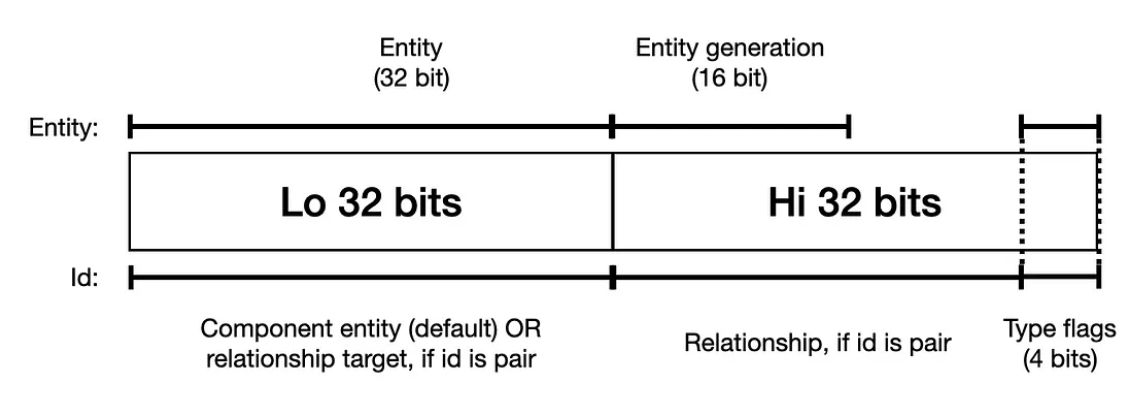
\includegraphics[width=0.5\linewidth]{resources/entity_generation.png}
    \caption{Smart Entity Generation in FLECS}
    \label{fig:entity_generation}
\end{figure}

% https://ajmmertens.medium.com/doing-a-lot-with-a-little-ecs-identifiers-25a72bd2647
Later in the paper, there will be mentions of a popular ECS framework called FLECS \textnormal{(Fast Lightweight Entitiy Component System)}. FLECS is unique in that it makes their ID generator more intelligent to decrease query times and grant the ability to define components at runtime with a technique called runtime tagging. The way IDs lower query times is by storing entity relationships inside the top half bits and the actual entity id in the lower half. The same technique is used to create entities with empty components, also known as tags, to the ID.  

\subsubsection{Component}
Similar to ENTITIES, the list of unique components is stored in the REGISTRY. The REGISTRY contains ID's that can be used as keys to access the COMPONENTS map. The COMPONENTS map then map's unique component ID's to homogenous component data. 

\subsubsection{System}
Systems can be registered to the SYSTEMS vector by providing two arguments: the set of components to iterate on and a function pointer to initiate the system. When the ECS world progresses by 1 tick, each system will have ran once.

\subsubsection{From Entitiy \textrightarrow{} Component}
In order to load the components of a given entity, the RECORD map is used. This map keeps track of the positions of components inside a homogenous component vector. Although this may be the case, a keen observer may notice how much more lookup is needed to load a single entity versus an entire component. \\

In order to load a specific entity, the ECS must:

\begin{enumerate}
    \item Check the Entity RECORD.
    \item Load the following components in COMPONENTS.
    \item Load the offsets in each component.
    \item Return to user.
\end{enumerate}

In order to load a specific component:

\begin{enumerate}
    \item Load the registery.
    \item Load the following component.
    \item Return to user.
\end{enumerate}

% TODO: source
This instinctively feels like a heavy tradeoff but in real-time simulations it's unlikely that there will be more direct entity queries versus batch component queries.


\subsubsection{System Queries}
An important detail is omitted from this diagram: the way a system queries for entities and components. This detail is omitted in this example because the structure is simple enough to hand query abilities directly to the developer. Since this example only runs in single threaded contexts there is no need to overcomplicate it.

% https://github.com/SanderMertens/ecs-faq
\subsection{Existing ECS And Implementation Styles}
As shown in the previous section, the definition of an ECS gives many different ways to implement it into an architecture. The following are a brief overview of different ECS architectures seen in various real implementions. The concurrent model this paper proposes falls under the category of a Dense ECS.  

\subsubsection{Dense ECS}
\begin{figure}[htbp]
    \centering
    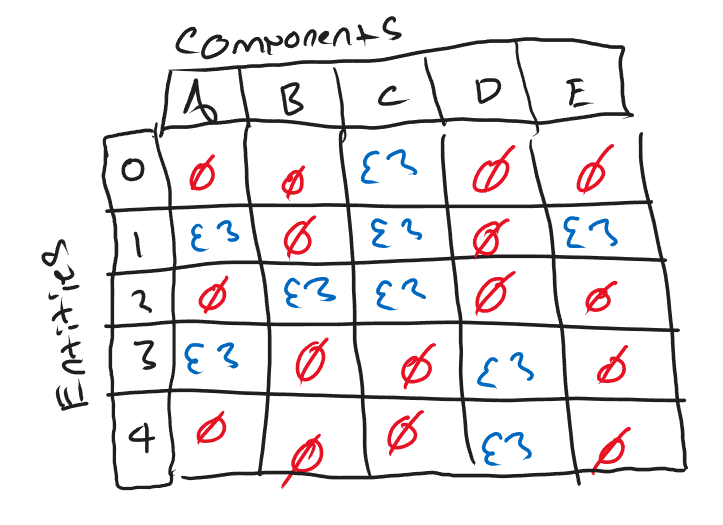
\includegraphics[width=0.5\linewidth]{resources/dense_ecs.png}
    \caption{Dense ECS Architecture Example}
    \label{fig:dense_ecs}
\end{figure}

A dense ECS stores entities in tables, where components are columns and entities are rows. This gives way for fast queries and easy to iterate over. Some popular examples of this type of ECS is FLECS and Unity's own ECS, Unity DOTS.

\subsubsection{Sparse ECS}
% https://programmingpraxis.com/2012/03/09/sparse-sets/
% https://citeseerx.ist.psu.edu/viewdoc/summary?doi=10.1.1.30.7319
% https://research.swtch.com/sparse 
Before discussing sparse ECS architectures, a small introduction into sparse sets is necessary. They are a datastructure dedicated to keeping the invariance of the following property:
\begin{equation*}
    \forall v \in \{0,\ldots, n-1\} : \text{D}[S[v]] = v
\end{equation*}
In the property above, $D$ and $S$ represent two vectors. The dense vector and sparse vector respectively. By using these two vectors in unison: lookup, insertion, and deletion time are all $O(1)$ and iteration is $O(n)$. 

% https://skypjack.github.io/2019-03-21-ecs-baf-part-2-insights/
% TODO: source https://www.flecs.dev/flecs/md_docs_2FAQ.html#:~:text=When%20you%20are%20comparing%20Flecs,queries%20are%20faster%20in%20Flecs
% https://github.com/SanderMertens/ecs-faq?tab=readme-ov-file
The main advantage of the sparse ECS is how fast it is to teest if an entity contains a component. Because of this, sparse ECS's advantages come in the form of query optimization. In a sparse ECS, a query iterates over all entities with the first queried for component, then takes that set and tests each subsequent component if every entity has it. Bitset ECS's are known to use similar approaches in their implementations.

Sparse sets also have another use where systems own their own sparse sets and they are kept to date each tick during runtime. These system owned sparse sets are then used to collect entities related to the system. An example of an ECS that does this technique is ecst. 

Overall, it's important to know that sparse set ECS's are popular in situations where fast add/remove of single component operations are preferred over efficient batch operations. To back this claim, FLECS which is a popular dense ECS published its own benchmarking data against other wide-industry used ECS's. From their data, FLECS has slower add/remove operations then EnTT, a popular sparse set based ECS. Regardless of the advantages and disadvantages of using sparse vs dense ECS's, it can be summed up nicely by the creator of EnTT:

\begin{quote}
    \textbf{It’s a matter of taste}, in fact.
        - Michele Caini
\end{quote}

\subsubsection{Bitset-based}
A bitset-based ECS stores components in arrays such that the entity id is emulated as the index. It then uses a bitset to indicate which components an entity has in table where the index is the entity. Some examples of bitset implementations are EntityX and Specs.

\subsubsection{Reactive}
A reactive ECS is more different than the others in this list. A reactive ECS uses signals emitted from mutating entities to keep individual lists of which entities belong to which system. Entitas is an example of this. 

\subsection{Concurrency in ECS Implementations}
The majority of ECS implementations I investigated had trivial or very basic concurrency support.
% https://github.com/SanderMertens/flecs/issues/281

The example of one I did find was that of FLECS. The concurrency model in FLECS is simple. The user initally sets the amount of worker threads manually, and entities matched with a system will be divided equally across threads. 
This system is not ideal because performance is left at the table. If the model allowed for individual read/write permissions the engine could open up to more performance gains.
 

% TODO: maybe add another section about how vectorization actually works in archetypes vs types?

\section{Concurrency Model}
\label{chap:2}
The following chapter introduces a formal concurrency model written of this papers own design. The core of the paper is the theory proposed here. The GECS Library uses this theory to orchestrate components to ensure an acceptable degree of wait-free concurrency. This concurrency model is of this papers own design. It's inspired by FLECS in the way that it vectorizes type compositions.

\subsection{Formal definition} \label{section:formal_definition}
We define the following called a world context to be a property that exists in an ECS: $W = (T, A, \delta, \Lambda)$ consisting of:
\begin{enumerate}
    \item A finite set of types $T$.
    \item A set of archetypes $A \subseteq \mathcal{P}(T)$, where $\mathcal{P}(T)$ denotes the power set of $T$.
    \item Some transition function $\delta : A \times T \rightarrow A$.
    \item A set of systems $(\lambda, \lambda_{req}) \in \Lambda$ such that $\lambda : W \rightarrow W^\prime$ and $\lambda_{req} \subseteq \mathcal{P}(T)$ representing the types required to initiate $\lambda$.
\end{enumerate}

\subsubsection{World Contexts}
$W$ represents the concept of a world, or one simulation, within the ECS. The ECS ensures that the following properties in context to worlds hold:

\begin{enumerate}
    \item An ECS may contain multiple worlds, but must have at least one.
    \item Only one world can be considered to be the "real" context.
    \item All worlds except one can be considered to be in the "simulation" context.
\end{enumerate}

At a very high level, the real context contains all vectorized data and the simulation context contains future operations to be applied to the real context that are not able to be done concurrently. Later in this chapter, the paper provides a proof as to why certain operations within this concurrency model cannot be done in parallel. 

This definition will later be used in this chapter to generate the entity finite-state-machine (FSM).

\subsubsection{Systems}
Systems are a tuple containing two properties: $\lambda$ and $\lambda_{req}$. $\lambda_{req}$ is a set of types that can be used to match $\lambda$ to archetypes. All archetypes that are super-sets to $\lambda_{req}$ get matched with an archetype.

The second part to systems is the $\lambda$ function. This function takes in a world context, either the real context or a simulated one, and applies a set of mutations and returns a copy. This altered copy is then used to merge all entity FSM's into the real context after some serialization point in the future.

\subsection{Types And Archetypes Relationships}
Until now, components were assumed to be stored in large, homogeneous vectors. This is great for cache locality, vectorizability, and is optimal for an ECS. But such a system when put in a runtime environment quickly falls apart, namely when composite type entities are introduced (entities with more than one component). 

Where should new entities get placed? In vector A or vector B? If the vectors are forced to be homogeneous, and an entity is included that only has A xor B, then the length of A and B are different. This is not ideal for SIMD, so we want to introduce a system that allows for the existence of composite entities, without losing out on vectorized operations.

Archetypes are a composition of types that exist within $\mathcal{P}(T)$. Archetypes, argued later in this chapter, are always able to maintain their vectorizability. Archetypes are critical for this concurrency model to work. They are the foundation on which what is able to be parallelized during the GECS runtime \cite{SanderMertensECS}.

\subsubsection{The ABC Problem}

The ABC Problem is a problem introduced by the FLECS creator Sander Mertens \cite{SanderMertensECS}. The problem demonstrates the effectiveness of Archetypes in component storage while retaining its vectorizability property -- and it's a good introduction to archetypes.

Suppose there exists a set of entities $E$ and $n = |E|$. Suppose $T := \{A,B,C\}$ and for each type $t \in T$, there exists a homogeneous vector containing elements of type $t$. Then, if all entities in $E$ have all components this is the following layout of the ECS in memory:

\begin{figure}[H]
    \begin{lstlisting}[
        language=Java,
        numbers=none
    ]
    A components[n];
    B components[n];
    C components[n];
    \end{lstlisting}
    \caption{Homogeneous ECS Components}
    \label{code:homogenous_ecs}
\end{figure}

In this ideal world, entity ID's can be emulated by simply being the index to the vectors. This is possible because the indexing property for this scenario $\forall t \in T : |t| = n$ holds. This ECS is positioned advantageously because all vectors are contiguous and therefore are vectorizable. This is only true because of the indexing property mentioned.

Suppose during runtime one of the entities at some index $k$ removes some component $t$. In such a situation, the defined indexing property is broken because not all vectors are of the same length and the gap in memory now means vector operations will be slow.

Sander Mertens uses this setup to prove that an ECS cannot vectorize homogeneous components efficiently at all. This is done by reviewing all situations in which homogeneous components are mutated to make vectorization impossible or difficult. By the end, he presents an elegant alternative called archetypes and proves that archetypes leads to some form of good vectorizability.

\subsubsection{Archetypes}
Simply put, an archetype is a set of types. Archetypes add a layer of abstraction on top of types so to make ECS queries vectorizable. Instead of creating homogeneous vectors based on types in $T$, we can create homogeneous vectors based on archetypes in $A$. 

\begin{figure}[H]
    \begin{lstlisting}[
        language=C
    ]
    A a[A_len];    /* Archetype {A} Part: "A" */

    A a[AB_len];   /* Archetype {A,B} Part: "A" */
    B b[AB_len];   /* Archetype {A,B} Part: "B" */

    A a[AC_len];   /* Archetype {A,C} Part: "A" */
    C c[AC_len];   /* Archetype {A,C} Part: "C" */
    \end{lstlisting}
    \caption{ECS Components With Archetypes $\{\{A\},\{A,B\},\{A,C\}\}$}
    \label{code:ecs_archetypes}
\end{figure}

Even though in Figure \ref{code:ecs_archetypes} those arrays are independent they do not have to be. In the GECS implementation, for example, all components of an archetype are interleaved into a contiguous array. So archetype storage looks more like that of Figure \ref{code:homogenous_ecs} than Figure \ref{code:ecs_archetypes}. Figure \ref{fig:composite} elaborates on what is meant by interleaved components. This is called the composite.


\begin{figure}[htbp]
    \centering
    \begin{verbatim}
Archetype X:                                                             
+---------+---------+-------------+---------+---------+-------------+---+
|Component|Component|Component    |Component|Component|Component    |   |
|A      8B|B      8B|C         16B|A      8B|B      8B|C         16B|...|
+---------+---------+-------------+---------+---------+-------------+---+
    \end{verbatim}
    \caption{Example Composite Vector Of Archetype X}
    \label{fig:composite}
\end{figure}

The composite vector can contain components of varying lengths. Component C is twice as large as Components A and B. Note that since archetypes are sets of types, archetypes $AB \equiv BA$ represent the same archetype.

\subsection{Representing Archetypes As An Entity Finite-State-Machine}
\label{sec:fsm_arc}
ECS applications are expected to handle operations over entities that can add, modify, or remove components. In the context of archetypes, this means being able to transition an entity between them. 

An example of such a situation is a game. Suppose all entities within the proximity of some point in space gain a tag component saying "buffed", but when they leave the proximity the tag component is removed. These types of state transitions may occur hundreds of times and need to be performant. 

\subsubsection{The Entity FSM}

A finite state machine emerges from using archetypes to organize entities in a specific way. If the addition and removal of components are considered as state transitions, then the following in Figure \ref{fig:graph1} represents existing archetypes during some ECS runtime. We define vertices to be archetypes in $W$ and edges to be entity transitions to adjacent archetypes.

As an example, suppose we have an ECS with the following properties:
\begin{align}
    T &= \{A,B,C,D\} \\
    A &= \{ \emptyset, [A] , [A,C] ,[B], [A,B], [A,B,C], [B,D], [D]\} \\
    \Lambda &= \emptyset
\end{align}
                                    
\begin{figure}[htbp]
    \centering
    \begin{verbatim}
                      +---------+       +---------+                                  
        +------------>+   [A]   |<----->|  [A,C]  |<--------+                        
        |             +---------+       +---------+         |                        
        v                                    ^              v                        
   +---------+        +---------+            |         +---------+                   
   |   [ ]   |<------>|   [B]   | <----------+         | [A,B,C] |                   
   +---------+        +---------+                      +---------+                   
        ^                  ^  ^                             ^                        
        |      +---------+ |  |          +---------+        |                        
        +----->|   [D]   | |  +--------->|  [A,B]  +--------+                        
               +---------+ |             +---------+                                 
                           |  +---------+                                            
                           +->|  [B,D]  |                                            
                              +---------+                                            
    \end{verbatim}
    \caption{Example FSM Graph Of Archetypes During Runtime}
    \label{fig:graph1}
\end{figure}

As shown in Figure \ref{fig:graph1}, all graphs contain the empty set $\emptyset$ as a vertex. This is because all entities when initiated contain the archetype with no components. As components get added to entities over their runtime, entities perform state transitions to their designated archetype.

It's important to remember that a serialization point is when the tick increments. All state transitions and entity states before the serialization point are considered invalid. Because of this, we know that entities require only one real transition per tick to a valid state. 

This means an entity could perform the transition, say $\{B,D\} \rightarrow \{A,B,C\}$ in one step, even though it passes through archetypes $[\{B\}, \{A,B\}]$ on the FSM. On the next tick, the edge $\{B,D\} \rightarrow \{A,B,C\}$ will be present. 

Entity Finite State Machines display the following properties:

\begin{enumerate}
    \item All existing archetypes must have a path to vertex $\emptyset$.
    \item Components can appear multiple times.
    \item Archetypes can only appear once.
    \item Entities can only appear once at one archetype.
\end{enumerate}

There are a couple interesting things to notice in Figure \ref{fig:graph1}. Notice how there is no transition between state $[B,D]$ and $[D]$. This is because this graph represents a runtime of an ECS and while it is possible to transition between $[B,D] \leftrightarrow [D]$, it has yet to happen in this runtime context, and is therefore not required to exist. 

The component $C$ in Figure \ref{fig:graph1} is special in the regard that it is not adjacent to the $\emptyset$ vertex like the others. This does not mean that it is impossible to create an entity with only component $C$ but that the runtime has yet to have that situation occur.

To loop back to the proximity example in the introduction in section \ref{sec:fsm_arc}, by representing additions and deletions as runtime state transitions it should now be clear that large performance gains are achieved via these edges. Initially, the first entity that transitions between two states in the simulation will be slow because the edge between those two vertices must be made. Once that edge is made, it is cached and the deletion and transfer of an entity to another archetype drops from $O(N)$ to $O(1)$.

\subsubsection{Operations On Entity FSM}
The following operations are all thread safe due to the scheduling algorithm explained in section \ref{sec:scheduling}. All implementation details are abstracted away except the operations directly done on the FSM. 

\textbf{Entity Creation:} All entities when created start at the $\emptyset$ vertex. All entities that exist here are not query-able.

\textbf{Entity Component Addition/Deletion:} Aside from the simple transition using an existing edge. When a component addition occurs, two operations are completed. Suppose the archetype we are currently in is at archetype $G$ and are attempting to add component $C$. This mean we are attempting to transition to archetype $G \cup \{C\}$. The two operations required for component addition are lookup and connection operation.

\begin{enumerate}
    \item If $G \cup \{C\} \not\in A$, then do step 2. Else do step 3.
    \item Create a new archetype $G \cup \{C\} \in A$. Apply component addition.
    \item Create the edge $G \leftrightarrow G \cup \{C\}$. Apply component addition.
\end{enumerate}

Both component addition and deletion use the same transition function $\delta$, so the component deletion operation is the same procedure.  

\textbf{Entity Deletion:} When an entity is marked for deletion, the archetype has the choice to either delete it now or wait to delete all entities together in a batch at some point in the future. Both of these strategies are thread safe. 

What happens when an archetype loses all its entities? While it would make sense for the archetype to be deleted from the graph since no entities are there, and it'll keep it mathematically pretty, there's not much theoretical reason as to why they should be kept. 

In practice though, there's a decently high probability that archetype will gain an entity again. Deleting those edges to archetypes with no entities will only slow down specific entity transition patterns. The memory usage of an empty archetype is also inconsequential and so there is no real trade-off of keeping it alive.

\subsection{Scheduling Systems}
\label{sec:scheduling}

Due to the nature that ECS follows principles in data-oriented design, these architectures have an advantage in concurrency contexts. The following section is about an algorithm designed in this paper to schedule systems concurrently in such a way they produce one valid serialization point per tick. Therefore, this algorithm does not guarantee that all entities will enter a system in any order or be processed in some order. Entities may be sent to the system seemingly at random.

\subsubsection{Scheduling Algorithm}
Before discussing the scheduling algorithm, we must define more strictly what functions are allowed to query in this architecture. Since archetypes and the state machine are abstracted away from the user, the set of rules for what is query-able and what is not should not be exposed to the user. The architecture must handle all query requests and attempt to parallelize as much as possible. 

Generally, if there exists an archetype that is the super-set of the query, then the query is OK. But asking a library user to only query in sets of existing archetypes is unreasonable. If the user, for example, in their render system wants to collect non-associated components \texttt{[Position, Score, Health]}, the ECS will fail. There is no archetype that holds these three random components together. This would make the query a super-set of archetypes and this use case must be handled in some manner that keeps the concurrency model valid. 

The way this scheduling algorithm solves this is by asking the user to always give the intersection of required types. For this example, suppose:
\begin{itemize}
    \item Player contains \texttt{[Position, Texture, Inputs, Health, Score]}
    \item Enemy contains \texttt{[Position, Texture, Health, Bullets Left]}
    \item Game Objects contain \texttt{[Position, Texture]}
\end{itemize}

The intersection between (Player $\cap$ Enemy $\cap$ Game Objects) is a \{\texttt{Position, Texture}\} component set. Therefore the render system should request only for the those two components. This will allow the ECS to correctly queue up each of those entities as concurrently as possible. 

But what about the other data? If I only query for \texttt{Position} and \texttt{Texture}, how will I access \texttt{Score} and \texttt{Health}? By applying the 4th property of the entity FSM: entities can only appear once at one archetype, we know that only one version of the entity can exist at one time. It is actually safe to load the rest of the entity data off the archetype when its time to process a queried entity. This is because we are guaranteed to be the only ones who have access to this entity at a given time. Any component that is hidden only needs to have their entity tested to see if that component is available for that entity.

With this in mind, the only function class allowed to be given to the scheduling algorithm from the user are functions whose requirements are a subset or equal to some archetype type set in $A$. The archetype concept can be blanketed away from the user by requesting all queries to contain the minimal intersection of types. The simple algorithm below assigns each function on the Entity FSM as such:

\begin{figure}[H]
    \begin{enumerate}
        \item For each $\lambda \in \Lambda$, do the following steps 2-3:
        \item Construct the set $x = \{\forall a \in A : \lambda_{req} \subseteq a \} \setminus \{\emptyset\}$.
        \item For each archetype in set $x$, mark that archetype to run $\lambda$.
        \item Schedule a unique thread for all archetypes.
        \item For each thread, run each system $\lambda$ that marked this archetype.
    \end{enumerate}
    \caption{Scheduling Algorithm}
\end{figure}

\textbf{Example:} The following is an example execution table based on the algorithm above.

\begin{figure}[H]
    \centering
    \begin{verbatim}
                                          Itr Step:                                          
                                          +--+--+--+                                         
                                  Typeset:|0 |1 |2 |                                         
                                  +-------+--+--+--+                                         
                                  |{A}    |L3|  |  |                                         
                                  +-------+--+--+--+                                         
                                  |{B}    |  |  |  |                                         
                                  +-------+--+--+--+                                         
                                  |{D}    |L4|  |  |                                         
                                  +-------+--+--+--+                                         
                                  |{A,B}  |L3|  |  |                                         
                    Systems:      +-------+--+--+--+                                         
                    Requirements: |{A,C}  |L1|L3|  |                                         
                    L1 = [A,C]    +-------+--+--+--+                                         
                    L2 = [B,C]    |{B,D}  |L4|  |  |                                         
                    L3 = [A]      +-------+--+--+--+                                         
                    L4 = [D]      |{A,B,C}|L1|L3|L2|                                         
                                  +-------+--+--+--+                                                                               
    \end{verbatim}
    \caption{Example Execution Table}
    \label{fig:exec_table}
\end{figure}

Each row in the table above represents a unique thread. Each thread takes however long it needs to finish a function before moving onto the next. Each thread does not need to wait for the other threads to finish. Although, once all archetypes have finished, then the tick is complete and is ready for the next tick. 

Another way to visualize the execution table is with colors and the FSM. The following is an example graph marked based on the scheduling algorithm.

\begin{figure}[H]
    \centering
    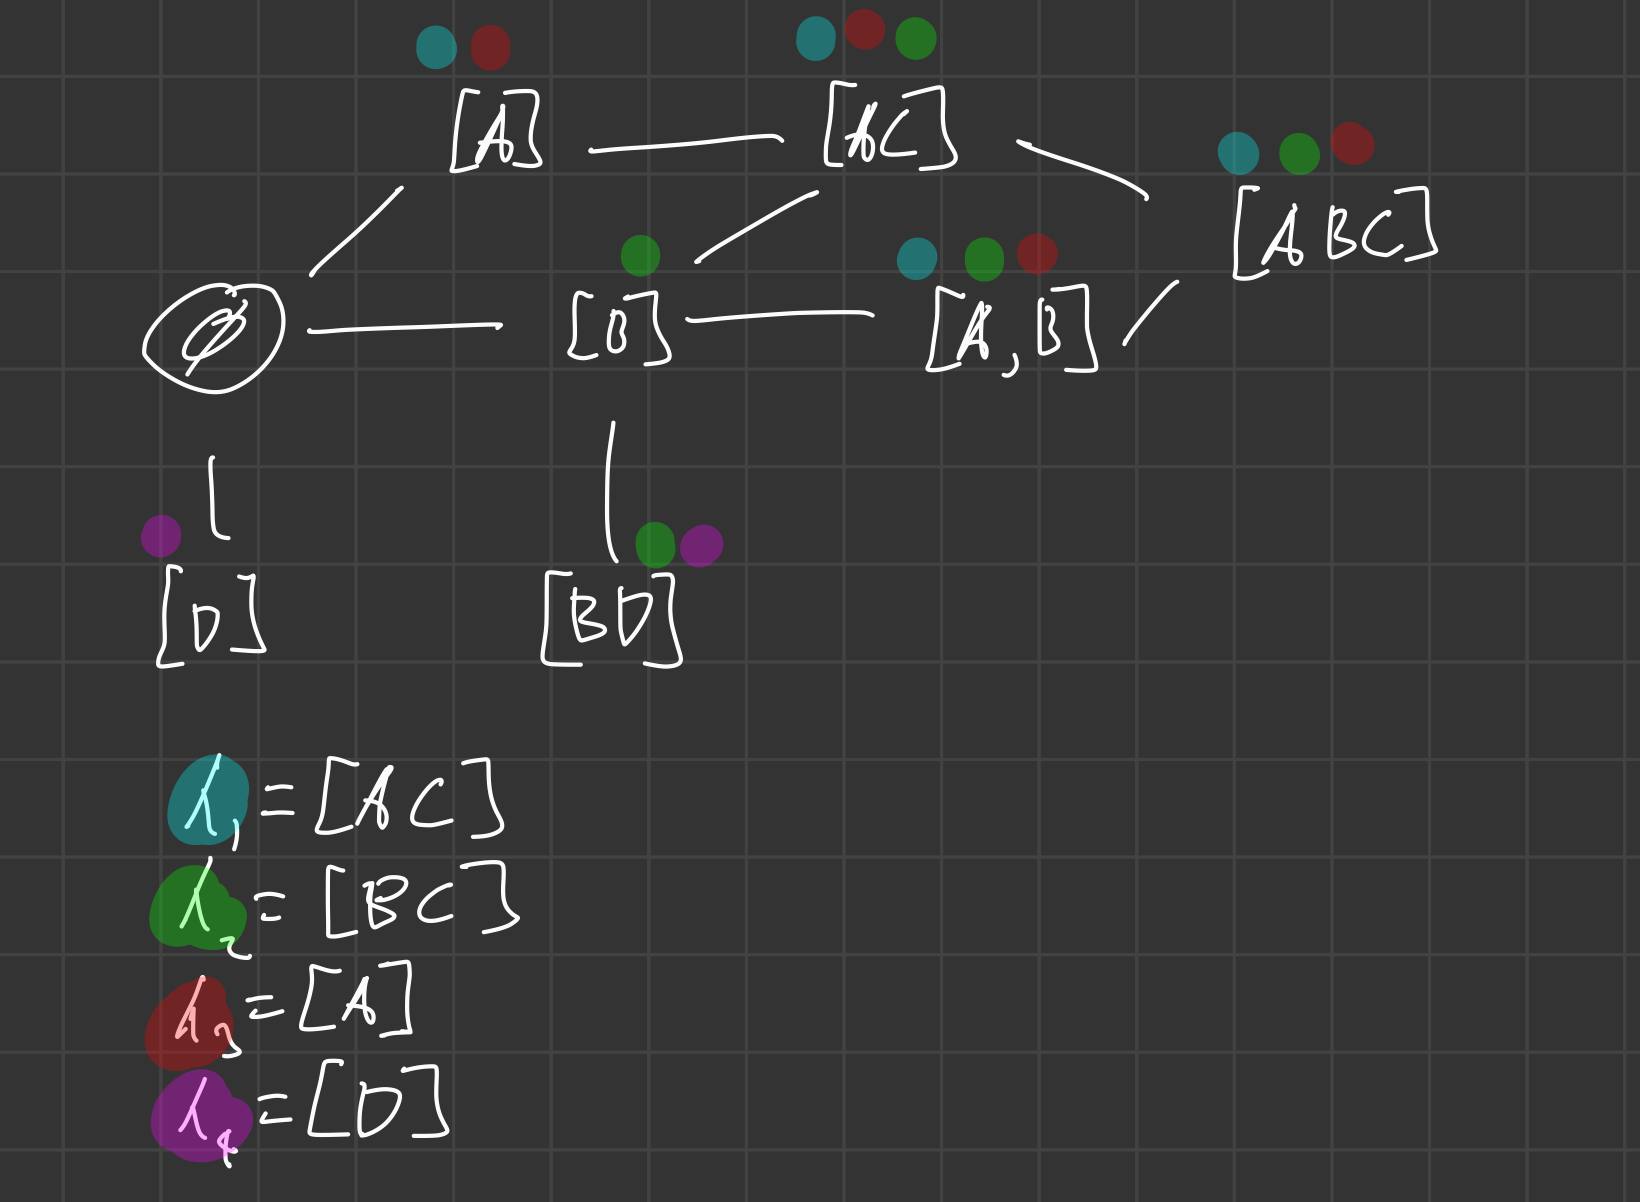
\includegraphics[width=0.8\linewidth]{resources/graph2.png}
    \caption{Example of a Scheduled Entity FSM Graph}
    \label{fig:graph2}
\end{figure}
 
Notice how on any archetype vertex in the graph when there are multiple colors signifies data access contention. Depending on ECS access patterns, an ECS could possibly squeeze a bit more performance but for most cases it is unnecessary. Although, the GECS implementation does provide support for embarrassingly parallel access patterns. So each $\lambda$ may also have some concurrency inside its own function.

\subsection{Entity Consolidation}
A key concept has been omitted thus far is entity consolidation. How, with these systems running concurrently, are entities transitioned between archetypes? It turns out that only entity and component reads/writes are able to be handled in parallel contexts. Component and entity creation/deletion cannot be handled in parallel contexts due to emerging non-determinism on the entity FSM.

The following sections contain a proof made for this paper and a workarounds is suggested.

\subsubsection{Entity Creation/Deletion Operations Leads To Tick Non-determinism}
\label{sec:proof1}
Suppose there exists two systems, systems A and B. Suppose entities live on an entity FSM that contains any set of states and includes some Type C. The purpose of System A is to generate new entities with Type C to place them on the FSM while the purpose of System B is to consume entities with Type C to remove them from the FSM. Both systems A and B run concurrently. 

In such an ECS runtime, entities are generated and transitioned to archetype $\{C\}$. Therefore, the count of entities at archetype $\{C\}$ while the tick is progressing.

There are three cases in which System A and B interact:
\begin{enumerate}
    \item System A generates entities faster than B consumes
    \item System A generates entities at the same rate B consumes
    \item System A generates entities slower than B consumes
\end{enumerate}

Only in case 3 can the next tick occur. The nondeterminism introduced by allowing entity list mutations on the finite state machine can cause program stalls such as in the manner proposed. What this means in a concurrent context is that this can lead to deadlocks, live-locks, or data invalidation.

The same sort of reasoning can be applied to only entity component creation and deletion as well.

\subsubsection{Serializability And Ledger-Based Consolidation}
\label{sec:ledger}
In order to solve the problem of entity consolidation in any context the entity list must stay fixed. That means for each tick, no matter the deletion or additions performed, the entity set must stay the same until the tick is complete. As such, even if perfect concurrent entity consolidation is performed, the effort is wasted. Instead of taking chances at doing concurrent insertions now, why not wait until the serialization point and save the effort? The performance will be the same due to the requirement of the list staying fixed. 

This model proposes to use a ledger-based consolidation technique that caches non-parallelizable operations done on the entity list and applies these operations after the serialization point. The GECS implementation uses separate entity FSM as caches.

\subsubsection{$\delta$ Transition To $\emptyset$}
Since entity deletion causes an entity to transition to $\emptyset$, it is not parallelizable and the fact this entity is deleted must be stored in the ledger. After the serialization point occurs, the ECS will go and clean out all entities that are supposed to translate to the $\emptyset$ directly from the ledger. 

\subsubsection{$\delta$ Transition To Non-$\emptyset$}
Much like the transition to the $\emptyset$, since the entity is transitioning archetypes it is not parallelizable. The transition operation will be stored in the ledger. After the serialization point, then the ECS will perform the $\delta$ transitions. 

\subsection{Model Properties}
The following discusses the two properties that the concurrency model exhibits. Its recursive nature and wait-free-ness. 

\subsubsection{Recursive Design}
\label{sec:recursive_design}
The entity FSM introduced above is only one part of the entire graph generated by an ECS. As stated previously in the definition, an ECS is a set of entity FSM's. 

Consider that each $\lambda$ system given by the user has the signature of $\lambda: W \rightarrow W^\prime$ where each $W^\prime$ represents a modified entity FSM based on $W$. Note that $\lambda$ returns a new structure that contains new entities and only old entities that got moved from their original archetype. This means that $W^\prime$ can represent a ledger of changes to be performed over $W$. It does not matter when these changes are applied to $W$, and there are advantages and disadvantages to processing these ledgers. Chaining these $\lambda$'s will produce a full recursive ECS graph, represented below.

\begin{figure}[htbp]
    \centering
    \begin{verbatim}
                            .     .     .         
                            .     .     .         
                            .     .     .         
                            ^     ^     ^         
                            |     |     |         
                            v     v     v         
                                                
                    ...  <-> W'<-> W <-> W''<-> ...
                                                
                            ^     ^     ^         
                            |     |     |         
                            v     v     v         
                            .     .     .         
                            .     .     .         
                            .     .     .         
    \end{verbatim}
    \caption{ECS graph connected via worlds generated by $\lambda$'s}
\end{figure}

This allows for a graph to naturally build out from $W$ where all edges contain changes to be performed on $W$. Letting a graph build out will in the short run make the engine process ticks faster at the expense of more cache misses later on and shorter vectorization lengths. Concurrency gains are expected to increase the larger the graph of ledgers gets, since simulated archetypes will run on their own thread.

\textbf{Why would this effect the vectorization lengths?} Since different $W$'s are allowed to contain the same archetype, entities over time will slowly be divided between different $W$'s and the original $W$. This means that the composite vector must share the count of entities that contain this typeset over two different vertices, so the lengths are shorter. 

\textbf{Why would this induce cache misses?} In the previous explanation it was discussed how archetype vertices on the FSM must share entities. Suppose this graph contains one system $\lambda$ and it's paired to archetype $A$. Suppose there are 100 entities existing on archetype $A$ before starting. If the graph is allowed to recursively grow for $N$ ticks, and $\lambda$ produces 10 entities, then it would take 10 ticks to produce 200 entities. The entity distribution among the graph looks like below:


\begin{figure}[htbp]
    \centering
    \begin{verbatim}
                        W --> W' --> W'2 --> ... W'10
                        ^     ^       ^           ^  
                        |     |       |           |
                        +---+ +-------+----+------+  
                        |                  |         
                        100          10               
                        Entities     Entities Each    
    \end{verbatim}
    \caption{Entity existing in identical archetypes on ledgers}
\end{figure}

If random access is performed across this set of worlds, cache misses are more likely than if all the entities lived on one archetype, one vector.

\textbf{Why will the concurrency gains increase by processing the ledgers?} Consider the same scenario above used to explain cache misses. Assume that entities all produced by $\lambda$ contain the same archetype signature as $A$, so that each entity is paired with archetype $A$. Using this, suppose it takes 1 second to process 1 entity. This means that $W$ would take 100 seconds and $\{W',\ldots,W^\prime 10\}$ would take 10 seconds each. 

We know that each archetype has its own thread, meaning that in total it would take only 110 seconds to process these entities. If this set of archetypes existing in the ledgers collapsed to $W$, then there would be 200 entities on archetype $A$ an thus take 200 seconds.

GECS does not do this due to thread management concerns and time constraints and spends significant time cleaning the ledger. There is also the concern of query times. For specific systems that exhibit recursive entity generation behaviors, they must be maintained in some manner to prevent the graph from over-growing and slowing down query performance. Due to these concerns, there are special limitations put in place in GECS to prevent recursive ledgers.

\subsubsection{Wait-Free In Model}
The entity FSM introduced in this chapter allows entities to be distributed over a graph and have each archetype perform whatever operations it want's to on this particular archetype without waiting or organizing between other archetypes. 

\section{GECS - Graph Entity Component System}
\label{chap:3}

\subsection{Data Layout And Data Structures}

\subsection{Examples}
\subsubsection{Basic}
\subsubsection{Concurrent}

\subsection{Entities}
\subsubsection{Representation}
\subsubsection{API}

\subsection{Components}
\subsubsection{Representation}
\subsubsection{API}

\subsection{Systems}
\subsubsection{Representation}
\subsubsection{API}


% \section{Benchmarks}
TBD
% \section{Discussion}
I am still working on benchmarks against other ECS's. Once that's ready I will write this section.
% \section{Conclusion \& Discussion}
The data presented in the previous section highlights a few key details and problems with the current implementation of the ECS. In the two tables provided in the descriptions section, show that the single threaded ECS is orders of magnitude faster than the multi-threaded one. Because the code between both models is shared except the concurrency, I believe this has to do with GECS creating and destroying threads within the game loop. This is in theory the only difference between both models. In order to perceive concurrency gain more clearly, further research is necessary as to why the threaded version is so slow and to create a thread pool that does not destroy and create threads dynamically. 

Even with various issues slowing it down, the engine did gain a tick-rate advantage when the simulation starts processing with more than 1024 entities per chunk. 

In summary, while the proposed wait-free ECS model shows promise and introduces an alternative approach, further work is necessary to refine its entity throughput. More ongoing research could lead to improvements to the efficiency of simulations, potentially influencing future developments. Regardless I view this project as a success when considering the research question was only if I could design a wait-free model in the context of ECS architecture. The model itself holds, and is able to accurately simulate as if any other ECS would. It offers the guarantee that the simulation will make progress within a finite number of steps.

\subsection{Known Performance Bottlenecks}
Looking back at this project, it's not surprising that the performance of GECS does not compete with the most popular ECS implementations. The following are features and parts of the code that in the future would bring large performance boosts. 

Throughout the code, all the TODO's listed are known performance bottlenecks. Many performance optimizations are as simple as instead of doing an iterative loop, a memmove call is possible. A lot of these optimizations were omitted to keep the programs complexity down, at least during core development.

\subsubsection{The CSDSA Library}
As mentioned before, the entire code stack is written by me, including all data structures and algorithms. For example, the built-in sort used for vectors at the moment is bubble sort. So whenever sorting N entities for the deletion algorithm, the sort is not $log(N)$ but $N^2$. Other more smaller things add up such as not having a good choice for a hashing function, so GECS experiences more collisions. Overall, if this engine was to compete, it should have used boost or Glib. 

\subsubsection{Unlock The Recursive Limiter}
Since this models main speed-up property is that each archetype runs it own thread, and that each archetype can recurse and make its own simulation, if we do not clean up the simulation every tick then there is a good amount of concurrent performance to gain.

GECS in its current state aggressively cleans up the simulation each tick which is unnecessary. Because of this, simulated archetypes cannot run concurrently as they do not have any entities at the beginning of all ticks, and therefore cannot make their own simulations. Section \ref{sec:recursive_design} offers an explanation on how unlocking recursion will potentially provide speed-ups.

\subsubsection{No Use Of SIMD}
There are obvious parts of the engine to me that should be using SIMD to do operations. An obvious one is the deletion algorithm. In theory, the subtraction between the vectors could be done in one vector operation.

\subsubsection{No Batch \& Concurrent Moves}
There are many internal parts of the engine that apply linear element-wise operations that could benefit from running concurrently or used over SIMD. A notable example is the defragmentation process. The two vectors are primed for SIMD since one subtracts the value from the other. This is foolishly done linearly.

\subsubsection{No Thread-pools}
For each archetype registered in GECS, it creates, spins up, and destroys the thread each iteration. This is terrible for performance and is most likely one of the key reasons why the engine is so slow with concurrency enable.

\subsubsection{Hashing Overuse \& Regex}
Every time any entity is accessed, the hash-name is re-calculated. This ended up being ridiculously expensive in the benchmark. Other libraries like FLECS, instead of constant ID look-ups, force you to cache the ID yourself to use in the call yourself. In hindsight, this would have decreased time in benchmarks quite a lot.

It was not a good idea to try using regex for matching. The current implementation, when doing any component operation, requests the type name of the component. This type name turns into a string with the C pre-processor. This string may contain 1 or more type names, so it will be in the form "Component A, Component B, Component C,...". Each component name must be extracted, and each component name is hashed individually. 

This means that all component operations not only require new hashes each time, but regex must also be loaded and processed.

\subsubsection{No Read/Write Specification}
The current implementation of GECS does not specify if a type is going to be used in a read or write context. By providing this, the engine could do a better job at queuing systems. Specifically in the game made for benchmarking, the objective was to provide 2 concurrent systems and one that queues up sequentially to do the logic. One of those systems is read only and the other is write only, but they contend the same data. So there was performance lost there.

\newpage

\printbibliography

\end{document}